%%%%%%%%%%%%%%%%%%%%%%%%%%%%%%%%%%%%%%%%%%%%%%%%%%%%%%%%%%%%%%%%%%%%%%%%%%
%%  PhD DEFENSE  --  Gabriel Jardanovski  --  Northwestern University
%%  Three essays:  (1) Inferring Emissions   ~10 min
%%                  (2) Carbon Leakage        ~10 min
%%                  (3) Carbon Policy in Networks (JMP) ~25 min
%%  Aesthetic cloned from the inferring_emissions beamer deck
%%  (metropolis + dove). Compile with xelatex.
%%%%%%%%%%%%%%%%%%%%%%%%%%%%%%%%%%%%%%%%%%%%%%%%%%%%%%%%%%%%%%%%%%%%%%%%%%
% !TEX program = xelatex
\documentclass[aspectratio=169]{beamer}

\usetheme{metropolis}
\usecolortheme{dove}

\usepackage{tikz}
\usetikzlibrary{positioning}
\usetikzlibrary{calc}
\usepackage{graphicx}
\usepackage{subfigure}
\usepackage{multirow}
\usepackage{booktabs}
\usepackage{adjustbox}
\usepackage{caption}
\usepackage{amsmath}
\usepackage{amssymb}
\usepackage{textcomp}
\usepackage{comment}
\usepackage{tcolorbox}
\usetikzlibrary{tikzmark,decorations.pathreplacing,calligraphy}
\usetikzlibrary{arrows}
\usetikzlibrary{decorations.markings}
\usetikzlibrary{shapes.misc}
\usetikzlibrary{matrix,shapes,arrows,fit,tikzmark, intersections}
\metroset{sectionpage=none}
\setbeamertemplate{frame numbering}[fraction]   % footer reads "x / N" (template style)
\usefonttheme[onlymath]{serif}
\usepackage{dcolumn}
\usepackage{tabularx}
\usepackage{color,xcolor,ucs}
\usepackage{bbm}

\newcolumntype{d}[0]{D{.}{.}{5}}

% ---- colorblind-friendly palette (same as inferring deck) ----
\definecolor{blue}{RGB}{0,114,178}
\definecolor{lblue}{rgb}{0.94, 0.97, 1.0}
\definecolor{red}{RGB}{164,42,4}
\definecolor{yellow}{RGB}{240,228,66}
\definecolor{green}{RGB}{0,158,115}
\definecolor{gray}{RGB}{240,240,240}
\definecolor{dgray}{RGB}{128,128,128}
\definecolor{purple}{RGB}{78,42,132}

\setbeamercolor{button}{bg=white, fg=blue}

\tikzset{place/.style={circle,thick,draw=blue!75,fill=blue!20,minimum size=10mm}}
\tikzset{place2/.style={circle,thick,draw=blue!75,fill=green!20,minimum size=10mm}}
\tikzset{place3/.style={circle,thick,draw=red!75,fill=orange!20,minimum size=10mm}}
\tikzset{main node/.style={circle,draw,font=\sffamily\small\bfseries,minimum size=10mm}}

\newenvironment{wideitemize}{\itemize\addtolength{\itemsep}{5pt}}{\enditemize}

% ---- alert colors ----
\newcommand<>{\alertb}[1]{\begingroup%
\setbeamercolor{alerted text}{fg=blue}\alert{#1}\endgroup}
\newcommand<>{\alerty}[1]{\begingroup%
\setbeamercolor{alerted text}{fg=yellow}\alert{#1}\endgroup}
\newcommand<>{\alertr}[1]{\begingroup%
\setbeamercolor{alerted text}{fg=red}\alert{#1}\endgroup}
\definecolor{lmugreen}{RGB}{0,148,64}
\newcommand<>{\alertg}[1]{\begingroup%
\setbeamercolor{alerted text}{fg=lmugreen}\alert{#1}\endgroup}
\definecolor{orange}{RGB}{255,127,0}
\newcommand<>{\alerto}[1]{\begingroup%
\setbeamercolor{alerted text}{fg=orange}\alert{#1}\endgroup}
\definecolor{webpurple}{rgb}{0.5,0,0.7}
\newcommand<>{\alertp}[1]{\begingroup%
\setbeamercolor{alerted text}{fg=webpurple}\alert{#1}\endgroup}
\definecolor{ochre}{RGB}{205,100,0}
\newcommand<>{\alertoch}[1]{\begingroup%
\setbeamercolor{alerted text}{fg=ochre}\alert{#1}\endgroup}

\setbeamercolor{frametitle}{bg=gray}
\setbeamercolor{progress bar}{fg=black,bg=black}

\setbeamercolor{block title alerted}{use={block title, alerted text}, bg=blue, fg=white}
\setbeamercolor{block body alerted}{use=block title, bg=white}
\setbeamerfont{block title alerted}{series=\mdseries}

\newenvironment{transitionframe}{
  \setbeamercolor{background canvas}{bg=gray}
  \setlength\lineskip{10pt}
  \begin{frame}[plain]}{
    \end{frame}
}

\newcommand{\ulg}{\textcolor{dgray}{\tiny$\blacktriangleright$}}
\usepackage{enumitem}

\setbeamertemplate{itemize items}{\ulg}
\setbeamertemplate{section in toc}[sections numbered]
\setitemize{label=\raisebox{.25ex}{\scriptsize\ulg}}

% ---- math macros shared with the papers ----
\newcommand{\N}{\mathcal{N}}
\newcommand{\U}{\mathcal{U}}
\newcommand{\Ntilde}{\tilde{\mathcal{N}}}

% ---- chapter-divider helper (template-style per-essay identity) ----
% #1 = accent color, #2 = chapter number, #3 = chapter title, #4 = co-authors / time
\newcommand{\chapterdivider}[4]{%
  \begin{transitionframe}
    \begin{center}
      \vspace{0.7cm}
      {\color{#1}\large\textbf{Chapter #2}}\\[0.6cm]
      {\color{#1}\Huge\textbf{#3}}\\[0.8cm]
      {\color{dgray}\normalsize #4}
    \end{center}
  \end{transitionframe}
}

%%%%%%%%%%%%%%%%%%%%%%%%%%%%%%%%%%%%%%%%%%%%%%%%%%%%%%%%%%%%%%%%%%%%%%%%%%
\title{Carbon Policy in Production Networks}
\subtitle{Three Essays on Emissions, Networks, and Climate Policy}
\date{}
\author{\textbf{Gabriel Jardanovski}}
\institute{\color{purple}{Northwestern University}}

\begin{document}

\tikzset{
        every picture/.style={remember picture,baseline},
        every node/.style={anchor=base,align=center,outer sep=1.5pt},
        every path/.style={thick},
        }

\maketitle

%%%%%%%%%%%%%%%%%%%%%%%%%%%%%%%%%%%%%%%%%%%%%%%%%%%%%%%%%%%%%%%%%%%%%%%%%%
%%  OVERVIEW
%%%%%%%%%%%%%%%%%%%%%%%%%%%%%%%%%%%%%%%%%%%%%%%%%%%%%%%%%%%%%%%%%%%%%%%%%%
{
    \setbeamertemplate{footline}{}
    \begin{frame}{Three essays on firms, emissions, and the production network}
        \begin{wideitemize}
            \item[\textbf{1.}] \alertg{\textbf{Inferring Firms' Emissions from Transactions Data}} \\
                {\color{dgray}\small \emph{measurement}: who emits, when emissions are unobserved? \hfill (\(\sim\)10 min)}

            \item[\textbf{2.}] \alertr{\textbf{Carbon Leakage Within and Across Countries}} \\
                {\color{dgray}\small \emph{reduced form}: does carbon pricing push activity to dirtier firms? \hfill (\(\sim\)10 min)}

            \item[\textbf{3.}] \alertb{\textbf{Carbon Policies in Production Networks}} \\
                {\color{dgray}\small \emph{structural}: how does \emph{who you cover} shape aggregate emissions? \hfill (\(\sim\)25 min)}
        \end{wideitemize}
        \vspace{0.4cm}
        \begin{center}
            {\color{dgray}\small A common thread: firm-level emissions and the buyer--supplier network,\\ measured in near-universal Belgian administrative data.}
        \end{center}
    \end{frame}
}

%%%%%%%%%%%%%%%%%%%%%%%%%%%%%%%%%%%%%%%%%%%%%%%%%%%%%%%%%%%%%%%%%%%%%%%%%%
%%  CHAPTER 1 -- INFERRING EMISSIONS
%%%%%%%%%%%%%%%%%%%%%%%%%%%%%%%%%%%%%%%%%%%%%%%%%%%%%%%%%%%%%%%%%%%%%%%%%%
\chapterdivider{green}{1}{Inferring Firms' Emissions\\ from Transactions Data}{with Gert Bijnens \quad$\cdot$\quad $\sim$10 minutes}
%%%%%%%%%%%%%%%%%%%%%%%%%%%%%%%%%%%%%%%%%%%%%%%%%%%%%%%%%%%%%%%%%%%%%%%%%%
%%  CHAPTER 1 -- INFERRING FIRMS' EMISSIONS FROM TRANSACTIONS DATA
%%  ~10 minutes. Frames lifted/trimmed from the inferring_emissions deck.
%%%%%%%%%%%%%%%%%%%%%%%%%%%%%%%%%%%%%%%%%%%%%%%%%%%%%%%%%%%%%%%%%%%%%%%%%%

%%%%%%%%%%%%%%%%%%%%% TEMPLATE-STYLE OVERVIEW %%%%%%%%%%%%%%%%%%%%%%%%%%%%
\begin{frame}{Inferring emissions: the problem in one slide}

    \begin{tcolorbox}[colback=green!5,colframe=green!40!black]
        \textbf{Question:} for the \emph{universe} of firms --- where emissions are
        unobserved --- how far can \textbf{B2B transaction data} take us in inferring
        firm-year emissions?
    \end{tcolorbox}

    \begin{wideitemize}
        \item[\alertg{Why hard:}] registries (EU ETS) \& surveys cover only \alertr{large installations}, in a handful of countries
        \pause
        \item[\alertb{Idea:}] firms that combust fossil fuels must \alerto{buy them} $\rightarrow$ purchases leave traces in the \alertp{transaction network}
        \pause
        \item[\alertoch{Data:}] Belgium --- near-universe B2B (2002--22) $+$ \alertg{verified EU ETS emissions} as ground truth
        \pause
        \item[\alertr{Result:}] a cross-fitted \alertp{elastic-net proxy} separates emitters from non-emitters (TPR 96\%, FPR $\le$17\%) and ranks them (Spearman $0.64$)
    \end{wideitemize}

\end{frame}

%%%%%%%%%%%%%%%%%%%%% TRAINING SAMPLE %%%%%%%%%%%%%%%%%%%%%%%%%%%%%%%%%%%%
\begin{frame}{Training sample: where the signal is learned}

    The set of firms we use to identify relevant suppliers:

    \begin{wideitemize}
        \item[\textbf{(i)}] \alertb{EU ETS firms}: 257 firms, 3,170 firm-years
        \begin{wideitemize}
            \item[-] verified yearly emissions from the EU Transaction Log
        \end{wideitemize}

        \item[\textbf{(ii)}] \alertg{Non-ETS firms in $\sim$100\%-covered sectors}: 2,959 firms, 23,438 firm-years
        \begin{wideitemize}
            \item[-] Petroleum refining (19), Iron \& steel (24), Paper, pulp \& print (17/18)
            \item[-] assigned \alerto{zero combustion emissions} (EU ETS covers $\sim$100\%)
        \end{wideitemize}
    \end{wideitemize}

    \vspace{0.3cm}
    \alertr{Why include the zeros?}
    $\rightarrow$ gives the model \alertb{extensive-margin} information;
    same sectors are \alerto{energy-intensive} $\Rightarrow$ a demanding test.

\end{frame}

%%%%%%%%%%%%%%%%%%%%% THE ELASTIC-NET APPROACH %%%%%%%%%%%%%%%%%%%%%%%%%%
\begin{frame}{Let the data identify the relevant suppliers}

    \begin{wideitemize}
        \item \alertb{Benchmark}: sum purchases from the six fuel-selling NACE codes
        \\ {\color{dgray}\small (Tabachova 2025, Stangl et al.\ 2026) --- misses multi-activity sellers, symmetric weights}

        \item \alertg{This paper}: regress verified emissions on \alertb{firm-year purchases from each supplier}
        $$ y_{it} = \sum_{j} \beta_j \, x_{ijt} + \gamma \log(\text{revenue}_{it}) + \boldsymbol{\delta}' \mathbf{d}_{t} + \boldsymbol{\phi}' \mathbf{s}_{i} + \varepsilon_{it} $$
        {\small $y_{it}=\operatorname{asinh}(\text{emissions})$, $x_{ijt}=\operatorname{asinh}(\text{sales})$; revenue \& FEs \alerto{unpenalized}}

        \item \alertp{Elastic-net penalty} on $\{\beta_j\}$ \;($\alpha=0.5$, $\lambda$ by firm-grouped CV)
        $\Rightarrow$ \alertb{EN-proxy}$_{it}=\!\!\sum_{j:|\hat\beta_j|>0}\!\!\hat\beta_j\,x_{ijt}$
    \end{wideitemize}

\end{frame}

%%%%%%%%%%%%%%%%%%%%% WHO ARE THE SELECTED SUPPLIERS %%%%%%%%%%%%%%%%%%%%
\begin{frame}{Who are the selected suppliers?}

    \begin{wideitemize}
        \item Out of $\sim$22,700 candidates, EN selects \alertb{612 suppliers} (463 $+$, 149 $-$)

        \item Dispersed across \alerto{53 NACE 2-digit sectors}:
        \begin{wideitemize}
            \item[-] largest: \alertp{wholesale trade (46)}; then construction, engineering, transport
            \item[-] \alertr{notably absent}: refined petroleum (19), electricity/gas (35)
        \end{wideitemize}

        \item Overlap with the NACE fuel-seller set is \alertr{minimal}: only \alertr{4 of 612} (0.7\%)

        \item[] \alertg{$\Rightarrow$ data-driven selection and NACE codes pick nearly disjoint sets of firms}
    \end{wideitemize}

\end{frame}

%%%%%%%%%%%%%%%%%%%%% EXTENSIVE-MARGIN VALIDATION %%%%%%%%%%%%%%%%%%%%%%%
\begin{frame}{The proxy separates emitters from non-emitters}

    \begin{columns}
    \begin{column}{0.6\textwidth}
        \begin{figure}
            \centering
            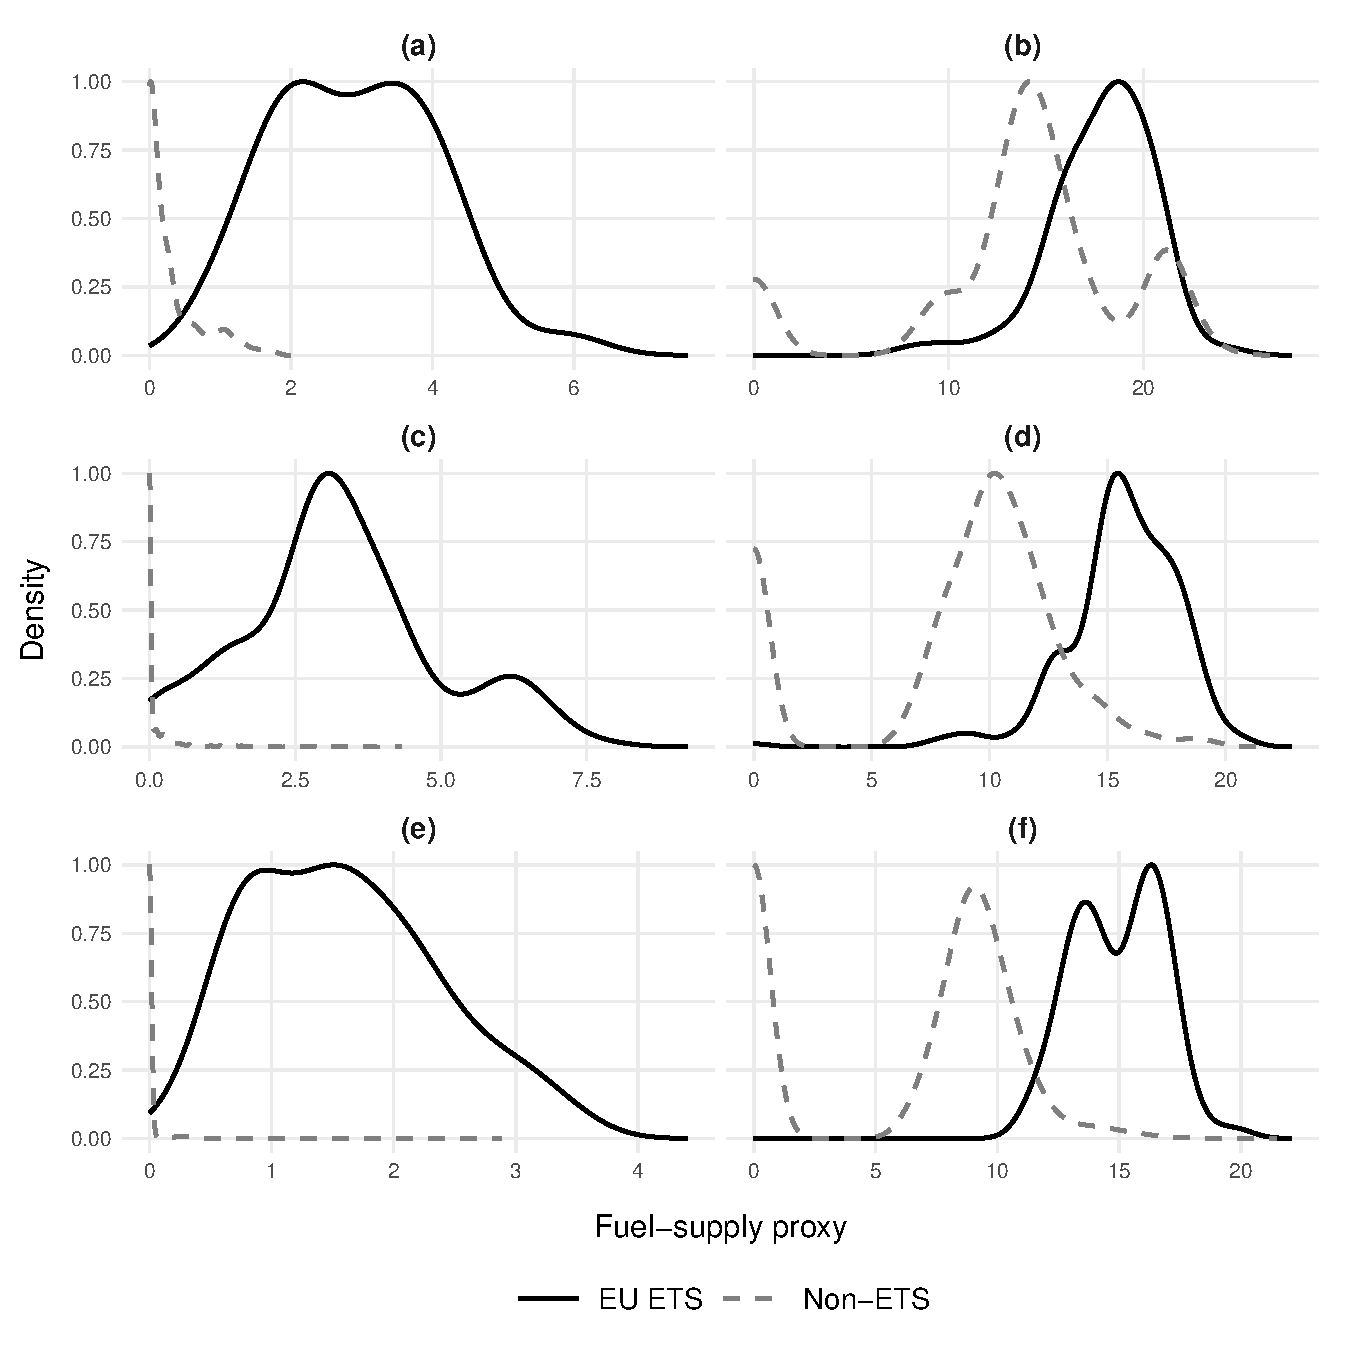
\includegraphics[width=\linewidth]{figures/proxy_density_by_emitter.pdf}
        \end{figure}
    \end{column}
    \begin{column}{0.4\textwidth}
        \begin{wideitemize}
            \item[] Kernel densities of the proxy
            \item[\alertb{Black}:] EU ETS firms
            \item[\alertr{Grey}:] non-ETS firms

            \item[]
            \item[] AUC (EN-proxy):
            \begin{wideitemize}
                \item[-] Petrol.\ ref.: \alertg{0.99}
                \item[-] Iron \& steel: \alertg{0.97}
                \item[-] Paper/print: \alertg{0.99}
            \end{wideitemize}
        \end{wideitemize}
    \end{column}
    \end{columns}

\end{frame}

%%%%%%%%%%%%%%%%%%%%% OUT-OF-SAMPLE RESULTS %%%%%%%%%%%%%%%%%%%%%%%%%%%%%
\begin{frame}{Out-of-sample performance (sector-level cross-fitting)}

    \begin{center}
    \scalebox{0.78}{
    \begin{tabular}{l ccc cc cccc}
    \toprule
     & \multicolumn{3}{c}{Prediction error} & \multicolumn{2}{c}{Correlation} & \multicolumn{4}{c}{Extensive margin} \\
    \cmidrule(lr){2-4} \cmidrule(lr){5-6} \cmidrule(lr){7-10}
     & RMSE & nRMSE & MAPD & Levels & Rank & FPR & TPR & p50 & p99 \\
    \midrule
    Revenue         & 190 & 1.00 & \alertg{0.71} & 0.85 & 0.53 & \alertr{1.00} & 1.00 & 0.01 & 0.39 \\
    Elastic Net     & 218 & 1.15 & 0.84 & 0.85 & \alertg{0.64} & \alertg{0.17} & 0.96 & 0.01 & \alertg{0.19} \\
    NACE            & 214 & 1.13 & 0.85 & 0.81 & 0.52 & 0.67 & 0.99 & 0.01 & 0.46 \\
    Gated Rev.\     & 193 & 1.01 & 0.71 & 0.84 & \alertg{0.68} & \alertg{0.17} & 0.96 & 0.00 & 0.35 \\
    Geom.\ Mean     & 218 & 1.15 & 0.74 & 0.83 & 0.63 & 0.26 & 0.97 & 0.01 & 0.28 \\
    \bottomrule
    \end{tabular}
    }
    \end{center}

    \begin{wideitemize}
        \item EN dominates the \alertg{extensive margin} (FPR $0.17$ vs.\ revenue $1.00$, NACE $0.67$)
        \item Revenue dominates \alertg{level accuracy among emitters} (MAPD $0.71$)
        \item \alerto{Gated Revenue} (EN classifies, revenue scales) $=$ best of both; rank corr.\ $0.68$
        \item[] {\footnotesize Means over $M=200$ sector-level CV repeats.}
    \end{wideitemize}

\end{frame}

%%%%%%%%%%%%%%%%%%%%% TAKEAWAYS %%%%%%%%%%%%%%%%%%%%%%%%%%%%%%%%%%%%%%%%%%
\begin{frame}{Chapter 1 --- takeaways}

    \begin{wideitemize}
        \item \alertb{B2B transaction data carry a signal about emissions} unavailable from balance-sheet variables alone

        \item A \alertp{cross-fitted elastic-net proxy} beats NACE classification, and a hybrid recovers the best of both margins

        \item \alertg{Broader lesson}: combustion $\Rightarrow$ fuel purchases $\Rightarrow$ network traces
        \begin{wideitemize}
            \item[-] a \alerto{general economic logic}, not Belgium-specific
            \item[-] testable wherever \alertp{transaction data $+$ a partial registry} coexist
        \end{wideitemize}

        \item[] {\color{dgray}\small $\hookrightarrow$ the same firm-level emissions \& network reappear, structurally, in Chapter~3.}
    \end{wideitemize}

\end{frame}


%%%%%%%%%%%%%%%%%%%%%%%%%%%%%%%%%%%%%%%%%%%%%%%%%%%%%%%%%%%%%%%%%%%%%%%%%%
%%  CHAPTER 2 -- CARBON LEAKAGE
%%%%%%%%%%%%%%%%%%%%%%%%%%%%%%%%%%%%%%%%%%%%%%%%%%%%%%%%%%%%%%%%%%%%%%%%%%
\chapterdivider{red}{2}{Carbon Leakage\\ Within and Across Countries}{with Gert Bijnens \quad$\cdot$\quad $\sim$10 minutes}
%%%%%%%%%%%%%%%%%%%%%%%%%%%%%%%%%%%%%%%%%%%%%%%%%%%%%%%%%%%%%%%%%%%%%%%%%%
%%  CHAPTER 2 -- CARBON LEAKAGE WITHIN AND ACROSS COUNTRIES
%%  ~10 minutes. 5 slides.  (numbers on slides 3 & 4 only)
%%%%%%%%%%%%%%%%%%%%%%%%%%%%%%%%%%%%%%%%%%%%%%%%%%%%%%%%%%%%%%%%%%%%%%%%%%

%%%%%%%%%%%%%%%%%%%%% (1) OVERVIEW %%%%%%%%%%%%%%%%%%%%%%%%%%%%%%%%%%%%%%%%
\begin{frame}{Carbon leakage within and across countries}

    \begin{tcolorbox}[colback=red!4,colframe=red!50!black]
        \textbf{Question:} does the EU ETS push activity toward \emph{less-regulated} suppliers ---
        \alertr{within} Belgium and \alertr{across} its borders?
    \end{tcolorbox}

    \begin{wideitemize}
        \item \textbf{\alertoch{Data:}} firm-level Belgium --- near-universe \alertb{B2B network} $+$ firm$\times$product$\times$country \alertp{customs} $+$ \alertg{EUTL} emissions/allowances
        \item \textbf{\alertb{Approach:}} continuous-treatment DiD --- dose $=$ a supplier's predetermined \alerto{carbon-cost exposure}; shock $=$ the \alerto{2015 MSR}-driven EUA run-up
        \item \textbf{\alertr{Result:}} carbon pricing \alertg{does} raise producer prices (more in exposed sectors) --- but sourcing \alertr{does not move}. \textbf{Three margins, three nulls.}
        \item \textbf{\alertp{Why:}} the relative-price gap stays \alertr{tiny} even at full pass-through --- too small to repay switching
    \end{wideitemize}

\end{frame}

%%%%%%%%%%%%%%%%%%%%% (2) PASS-THROUGH (+ SETTING) %%%%%%%%%%%%%%%%%%%%%%%
\begin{frame}{First: the policy \emph{does} bite on prices}

    \begin{columns}
    \begin{column}{0.55\textwidth}
        \begin{figure}
            \centering
            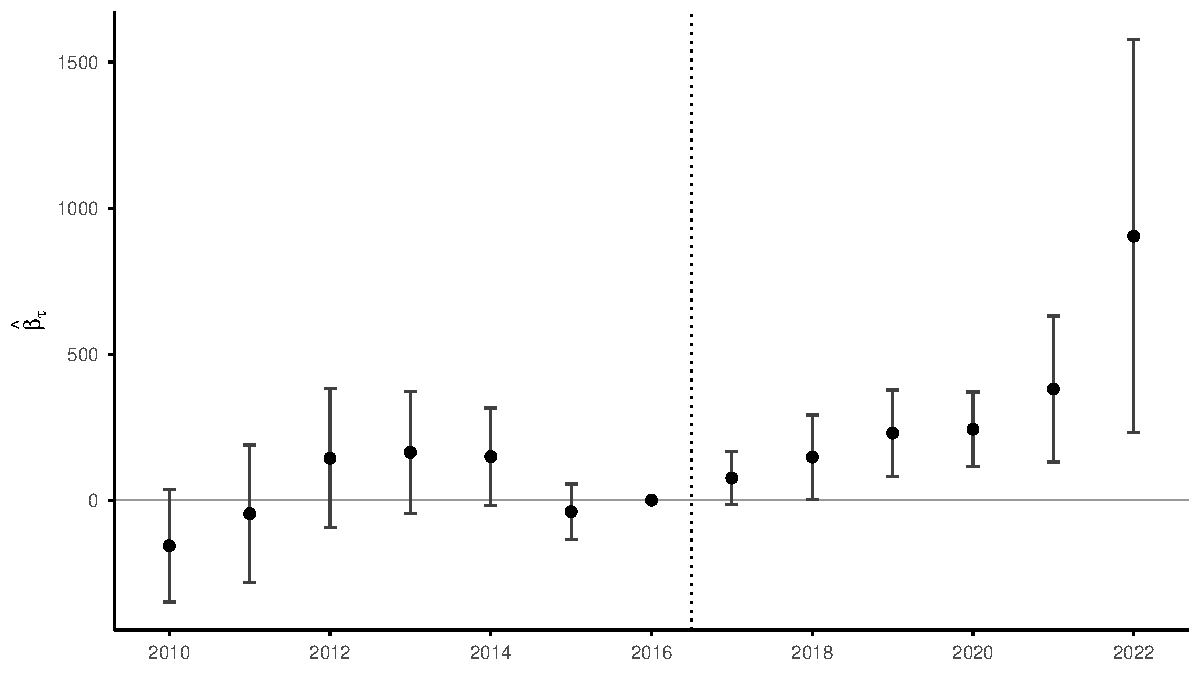
\includegraphics[width=\linewidth]{figures/phase4_ppi_eventstudy_omega_sh.pdf}
        \end{figure}
    \end{column}
    \begin{column}{0.45\textwidth}
        \begin{wideitemize}
            \item \textbf{\alerto{Shock}}: the 2015 MSR drives EUA \alertr{\texteuro5 $\to$ \texteuro80+} --- mechanical, predetermined
            \item \textbf{\alerto{Dose}}: supplier's pre-2017 exposure $\omega = \tfrac{\text{shortage}}{\text{total cost}}$
            \item Manufacturing prices rise after 2017 and \alertg{stay elevated}
            \item Concentrated in \alertb{shortage}-exposed sectors: \alertg{$+0.012^{**}\!\to\!+0.023^{***}$} per SD \\ {\footnotesize (gross emissions: \alertr{null})}
        \end{wideitemize}
    \end{column}
    \end{columns}

\end{frame}

%%%%%%%%%%%%%%%%%%%%% (3) DOMESTIC NULL (+ WHY) %%%%%%%%%%%%%%%%%%%%%%%%%%
\begin{frame}{Margin 1 --- within Belgium: no reallocation}

    \begin{columns}
    \begin{column}{0.55\textwidth}
        \begin{figure}
            \centering
            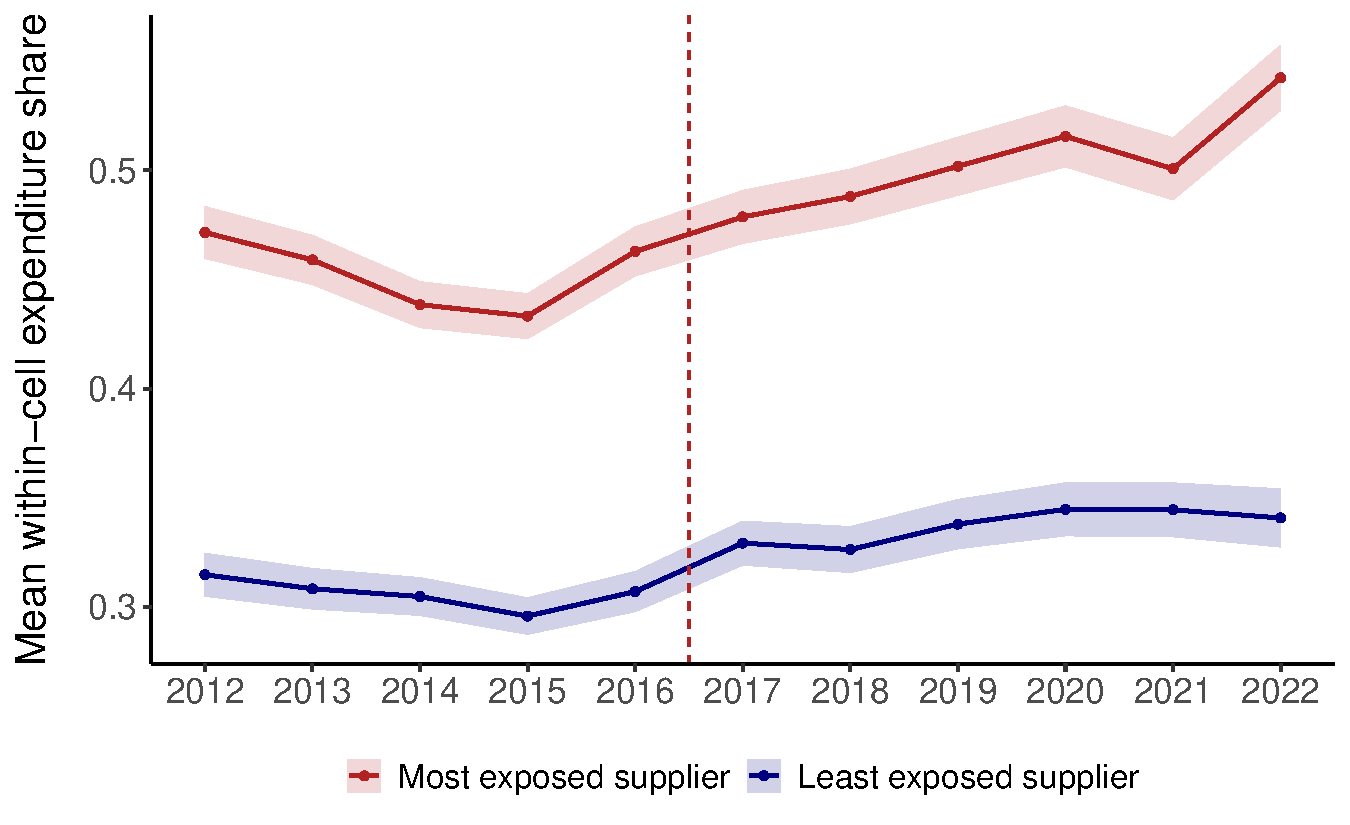
\includegraphics[width=\linewidth]{figures/phase4_within_nace4d_descriptive_trajectory_2017_activeAtT.pdf}
        \end{figure}
    \end{column}
    \begin{column}{0.45\textwidth}
        \begin{wideitemize}
            \item Expenditure share on \alertb{most-} vs.\ \alertr{least-}exposed supplier moves in \alertg{parallel} after 2017
            \item DiD on post$\times$top: \alertr{$+0.0123^{**}$} (wrong sign) $\to$ \alertg{$0.0031$ n.s.} once mechanical attrition is absorbed; not robust under HonestDiD
            \item \textbf{\alertb{Why}}: even at full pass-through the relative-price gap is \alertr{$<1\%$} --- too small to act on
        \end{wideitemize}
    \end{column}
    \end{columns}

\end{frame}

%%%%%%%%%%%%%%%%%%%%% (4) INTERNATIONAL NULL %%%%%%%%%%%%%%%%%%%%%%%%%%%%%
\begin{frame}{Margin 2 --- across borders: Belgium $\neq$ France}

    \begin{columns}
    \begin{column}{0.54\textwidth}
        \begin{figure}
            \centering
            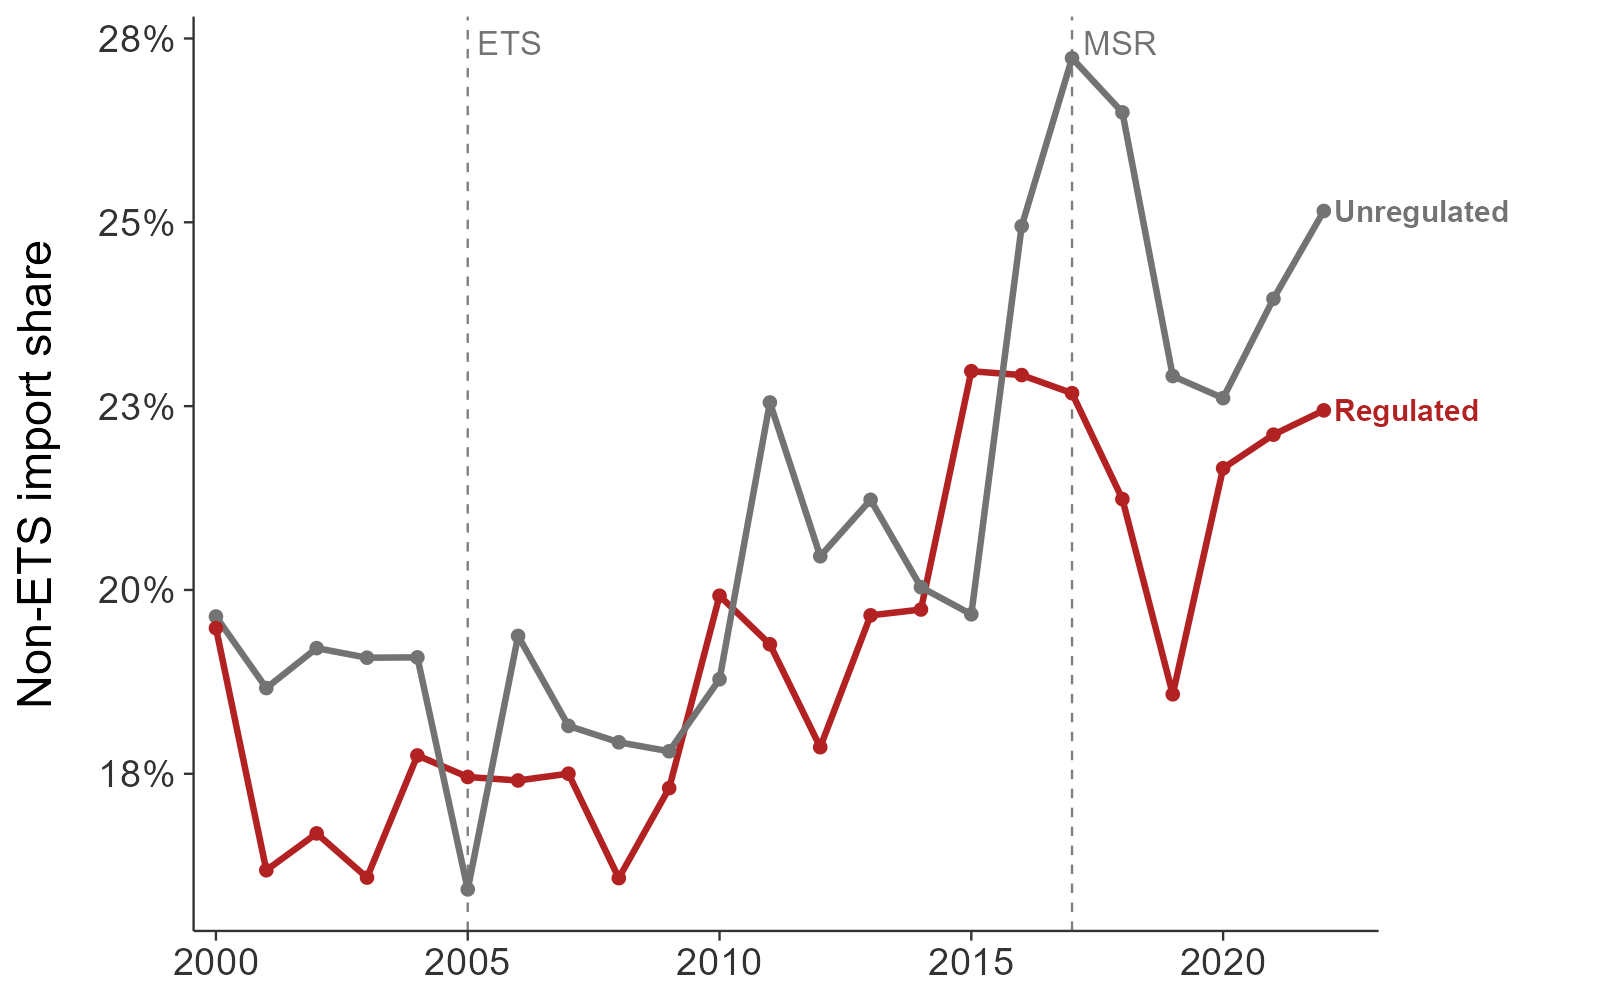
\includegraphics[width=\linewidth]{figures/phase2_cdgm_figure2_share.png}
        \end{figure}
    \end{column}
    \begin{column}{0.46\textwidth}
        \begin{wideitemize}
            \item Replicate Coster--M\'ejean--di Giovanni on Belgian customs: regulated imports, EU vs.\ non-EU sources
            \item Regulated $\times$ non-ETS share is \alertg{flat} across 2000--2022
            \item[] Intensive margin (value share):
            \begin{wideitemize}
                \item[-] Belgium: \alertr{$+0.0004$} (n.s.)
                \item[-] France: \alertb{$+0.121$} ($p<0.001$)
            \end{wideitemize}
            \item[] \alertp{$\Rightarrow$} a common EU carbon price need \alertr{not} produce the same leakage everywhere
        \end{wideitemize}
    \end{column}
    \end{columns}

\end{frame}

%%%%%%%%%%%%%%%%%%%%% (5) TAKEAWAYS %%%%%%%%%%%%%%%%%%%%%%%%%%%%%%%%%%%%%%%
\begin{frame}{Chapter 2 --- three margins, three nulls}

    \begin{tcolorbox}[colback=red!4,colframe=red!50!black]
        \centering The set of margins with detectable leakage is \textbf{empty}.
    \end{tcolorbox}

    \begin{wideitemize}
        \item[\alertg{1.}] Pass-through is \alertg{real} and persistent --- more in shortage-exposed sectors
        \item[\alertr{2.}] \alertr{No} within-NACE reallocation: wrong-signed, shrinks to insignificance, not robust
        \item[\alertr{3.}] \alertr{No} international reallocation: flat shares, far below France
    \end{wideitemize}

    \vspace{0.2cm}
    \alertp{Mechanism}: the cost shock is small and pass-through partial $\Rightarrow$ the relative-price gap never clears the cost of switching suppliers.

    \vspace{0.1cm}
    {\color{dgray}\small $\hookrightarrow$ Chapters 1--2 measure firms and test reallocation \emph{reduced-form};
    Chapter~3 builds the structural model that says \emph{when} reallocation should bind.}

\end{frame}


%%%%%%%%%%%%%%%%%%%%%%%%%%%%%%%%%%%%%%%%%%%%%%%%%%%%%%%%%%%%%%%%%%%%%%%%%%
%%  CHAPTER 3 -- CARBON POLICIES IN PRODUCTION NETWORKS (JMP)
%%%%%%%%%%%%%%%%%%%%%%%%%%%%%%%%%%%%%%%%%%%%%%%%%%%%%%%%%%%%%%%%%%%%%%%%%%
\chapterdivider{blue}{3}{Carbon Policies\\ in Production Networks}{Job Market Paper, with Gert Bijnens \quad$\cdot$\quad $\sim$25 minutes}
%%%%%%%%%%%%%%%%%%%%%%%%%%%%%%%%%%%%%%%%%%%%%%%%%%%%%%%%%%%%%%%%%%%%%%%%%%
%%  CHAPTER 3 -- CARBON POLICIES IN PRODUCTION NETWORKS (JMP)
%%  ~25 minutes. Equations & numbers verbatim from paper/thesis/.
%%%%%%%%%%%%%%%%%%%%%%%%%%%%%%%%%%%%%%%%%%%%%%%%%%%%%%%%%%%%%%%%%%%%%%%%%%

%%%%%%%%%%%%%%%%%%%%% TEMPLATE-STYLE OVERVIEW %%%%%%%%%%%%%%%%%%%%%%%%%%%%
\begin{frame}{Carbon policy in networks: the problem in one slide}

    \begin{tcolorbox}[colback=blue!4,colframe=blue!40!black]
        \textbf{Question:} a carbon price covers \emph{some} firms, not all. What is its
        effect on aggregate emissions, how does that depend on \emph{whom} it covers, and
        is there a firm whose coverage delivers the largest reduction?
    \end{tcolorbox}

    \begin{wideitemize}
        \item[\alertb{Theory:}] GE production network with heterogeneous emission intensities $+$ costly abatement; a carbon price $p_z$ and a $0/1$ coverage vector $\tau$
        \pause
        \item[\alertg{Result:}] $\dfrac{d\log Z}{dp_z}$ decomposes into \alerto{scale} ($\approx 0$), \alertp{technique} (abatement), and \alertb{reallocation} --- the last governed by a \textbf{single covariance} between a firm's policy exposure and its \emph{network-adjusted} emission intensity $\Psi_e$
        \pause
        \item[\alertoch{Data:}] Belgian B2B network $+$ EUTL $\Rightarrow$ under the EU ETS, the cut is \alertr{$\sim$7/8 abatement}, reallocation a modest amplifier
        \pause
        \item[\alertr{Punchline:}] $\sim$94\% of the gain from \emph{whom to cover} comes from firms' \alertr{own} emissions --- a constrained regulator just \alertb{targets the heaviest emitters}
    \end{wideitemize}

\end{frame}

%%%%%%%%%%%%%%%%%%%%% MOTIVATION 1: INCOMPLETE %%%%%%%%%%%%%%%%%%%%%%%%%%
\begin{frame}{Carbon pricing is incomplete by design}

    \begin{columns}
    \begin{column}{0.58\textwidth}
        \begin{figure}
            \centering
            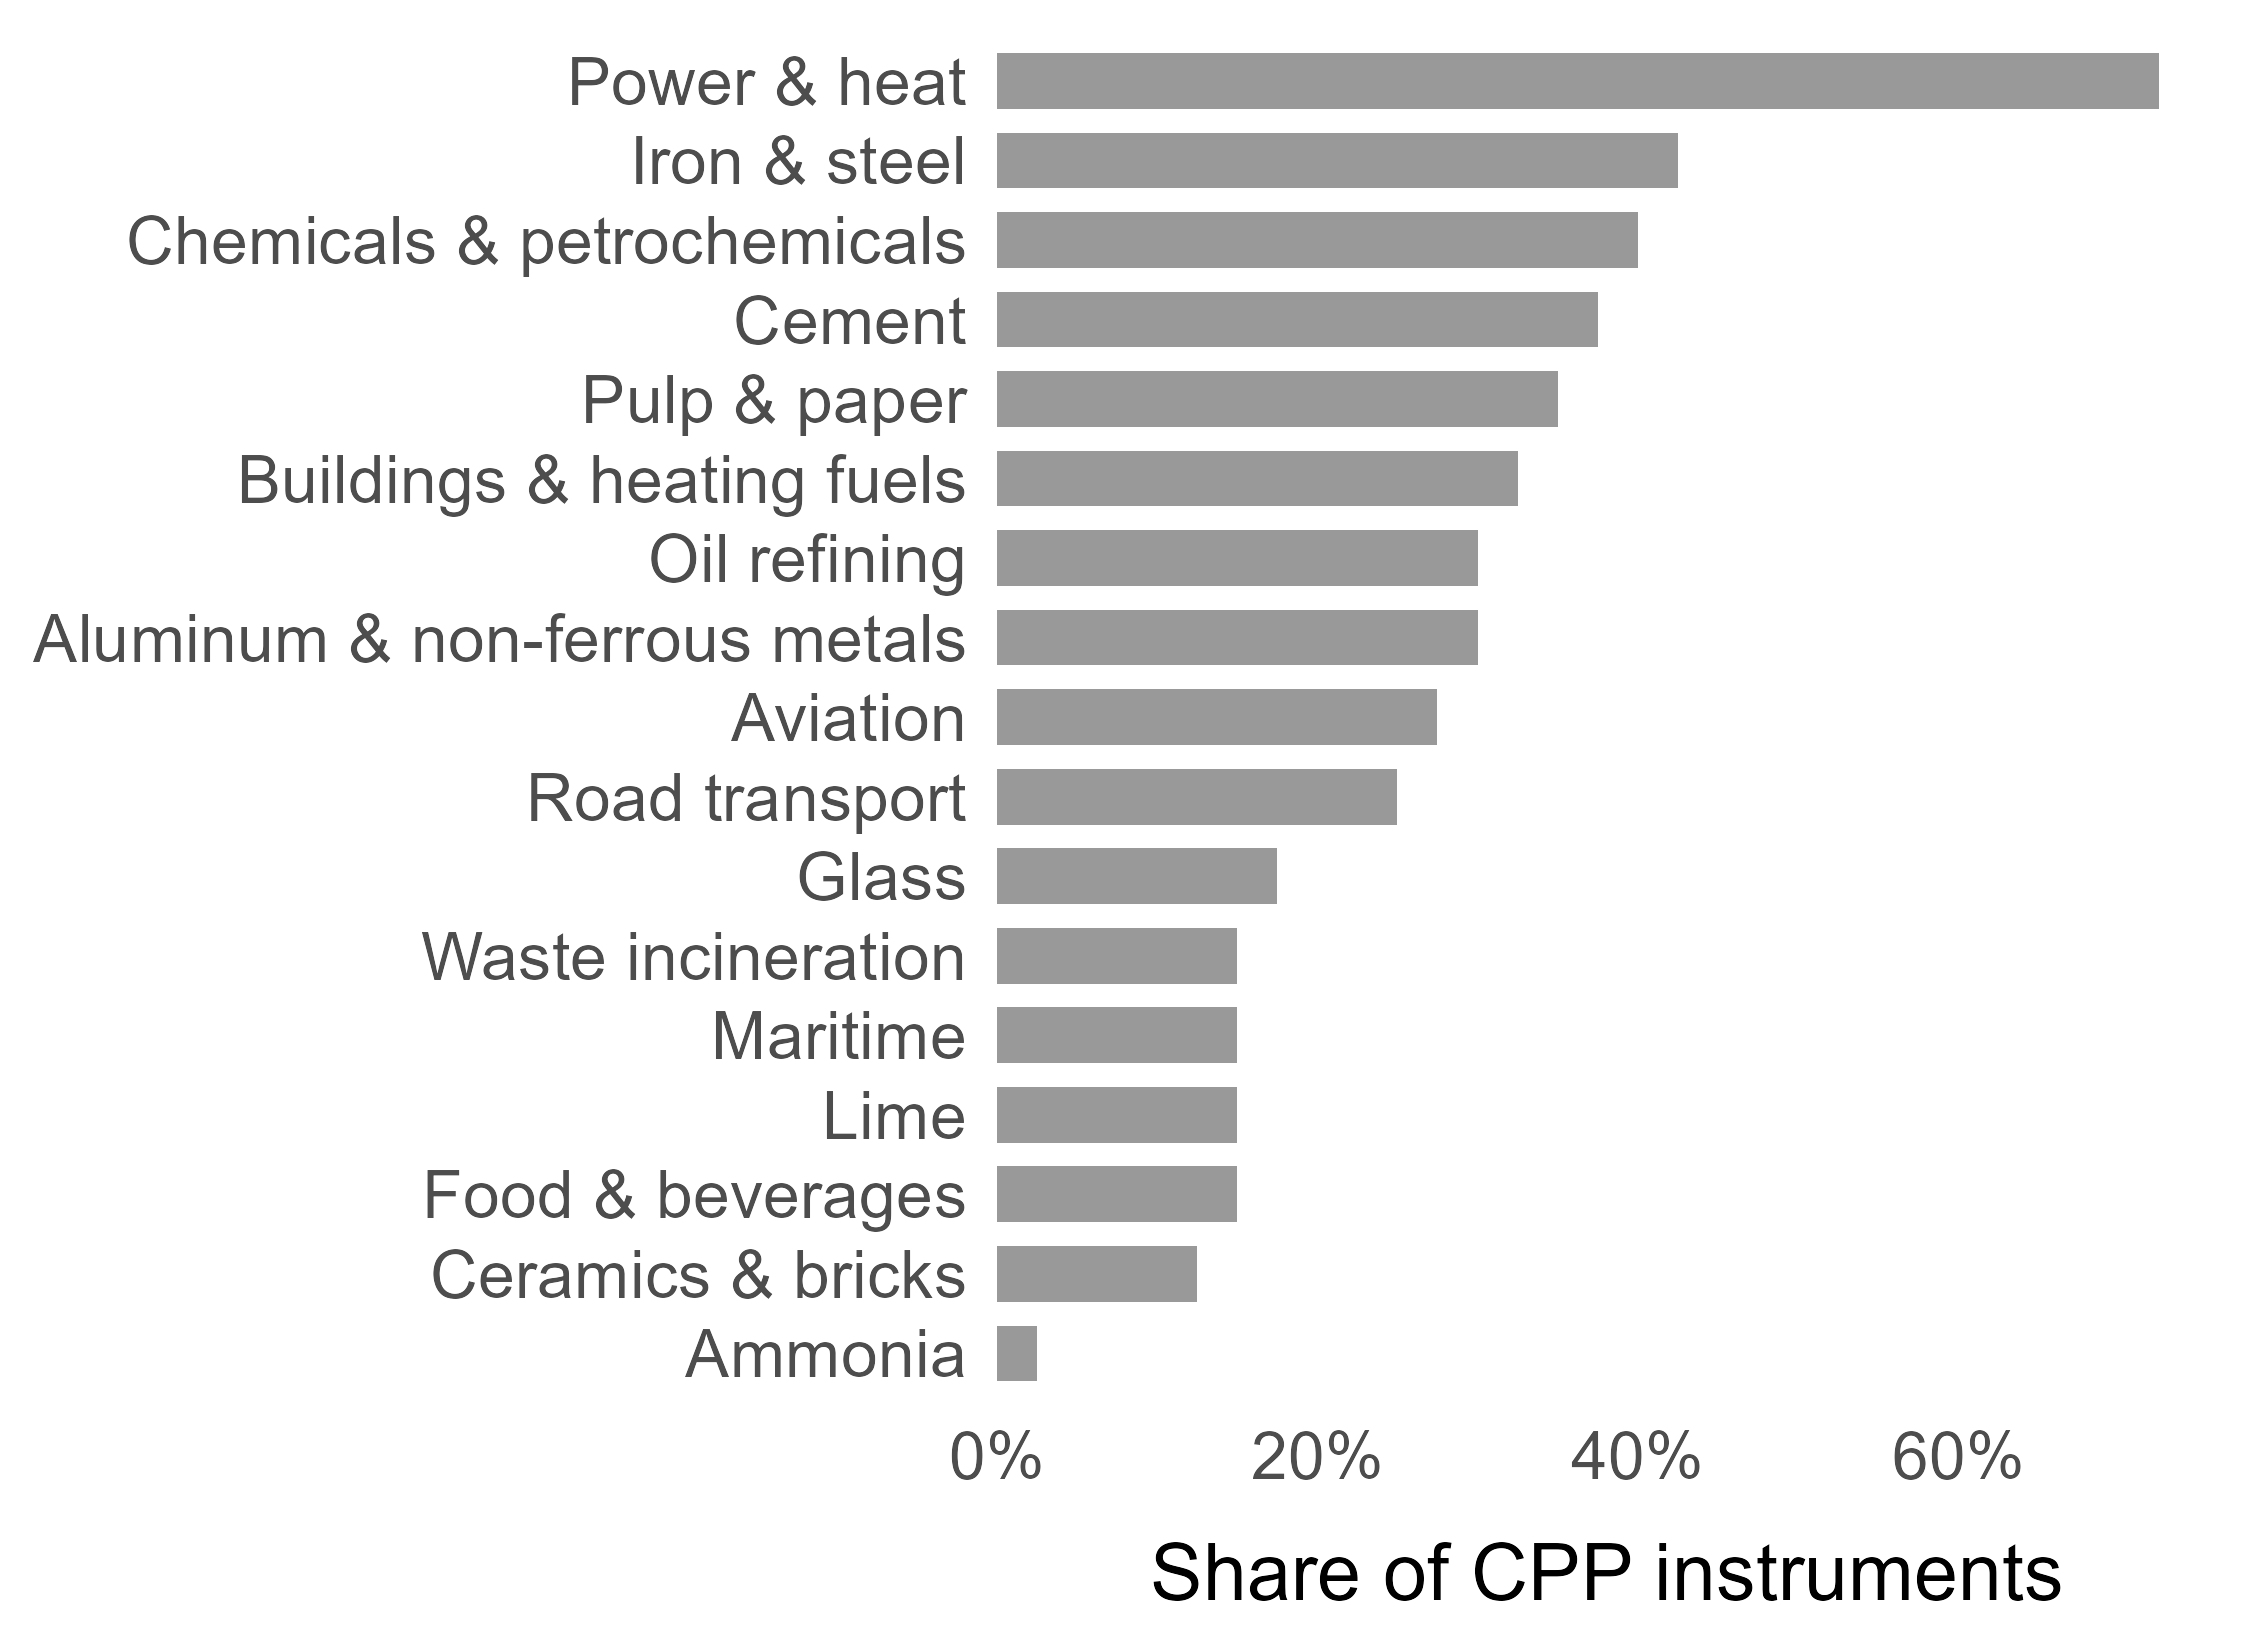
\includegraphics[width=0.99\linewidth]{figures/panel_a_sector_targeting.png}\\[0.2em]
            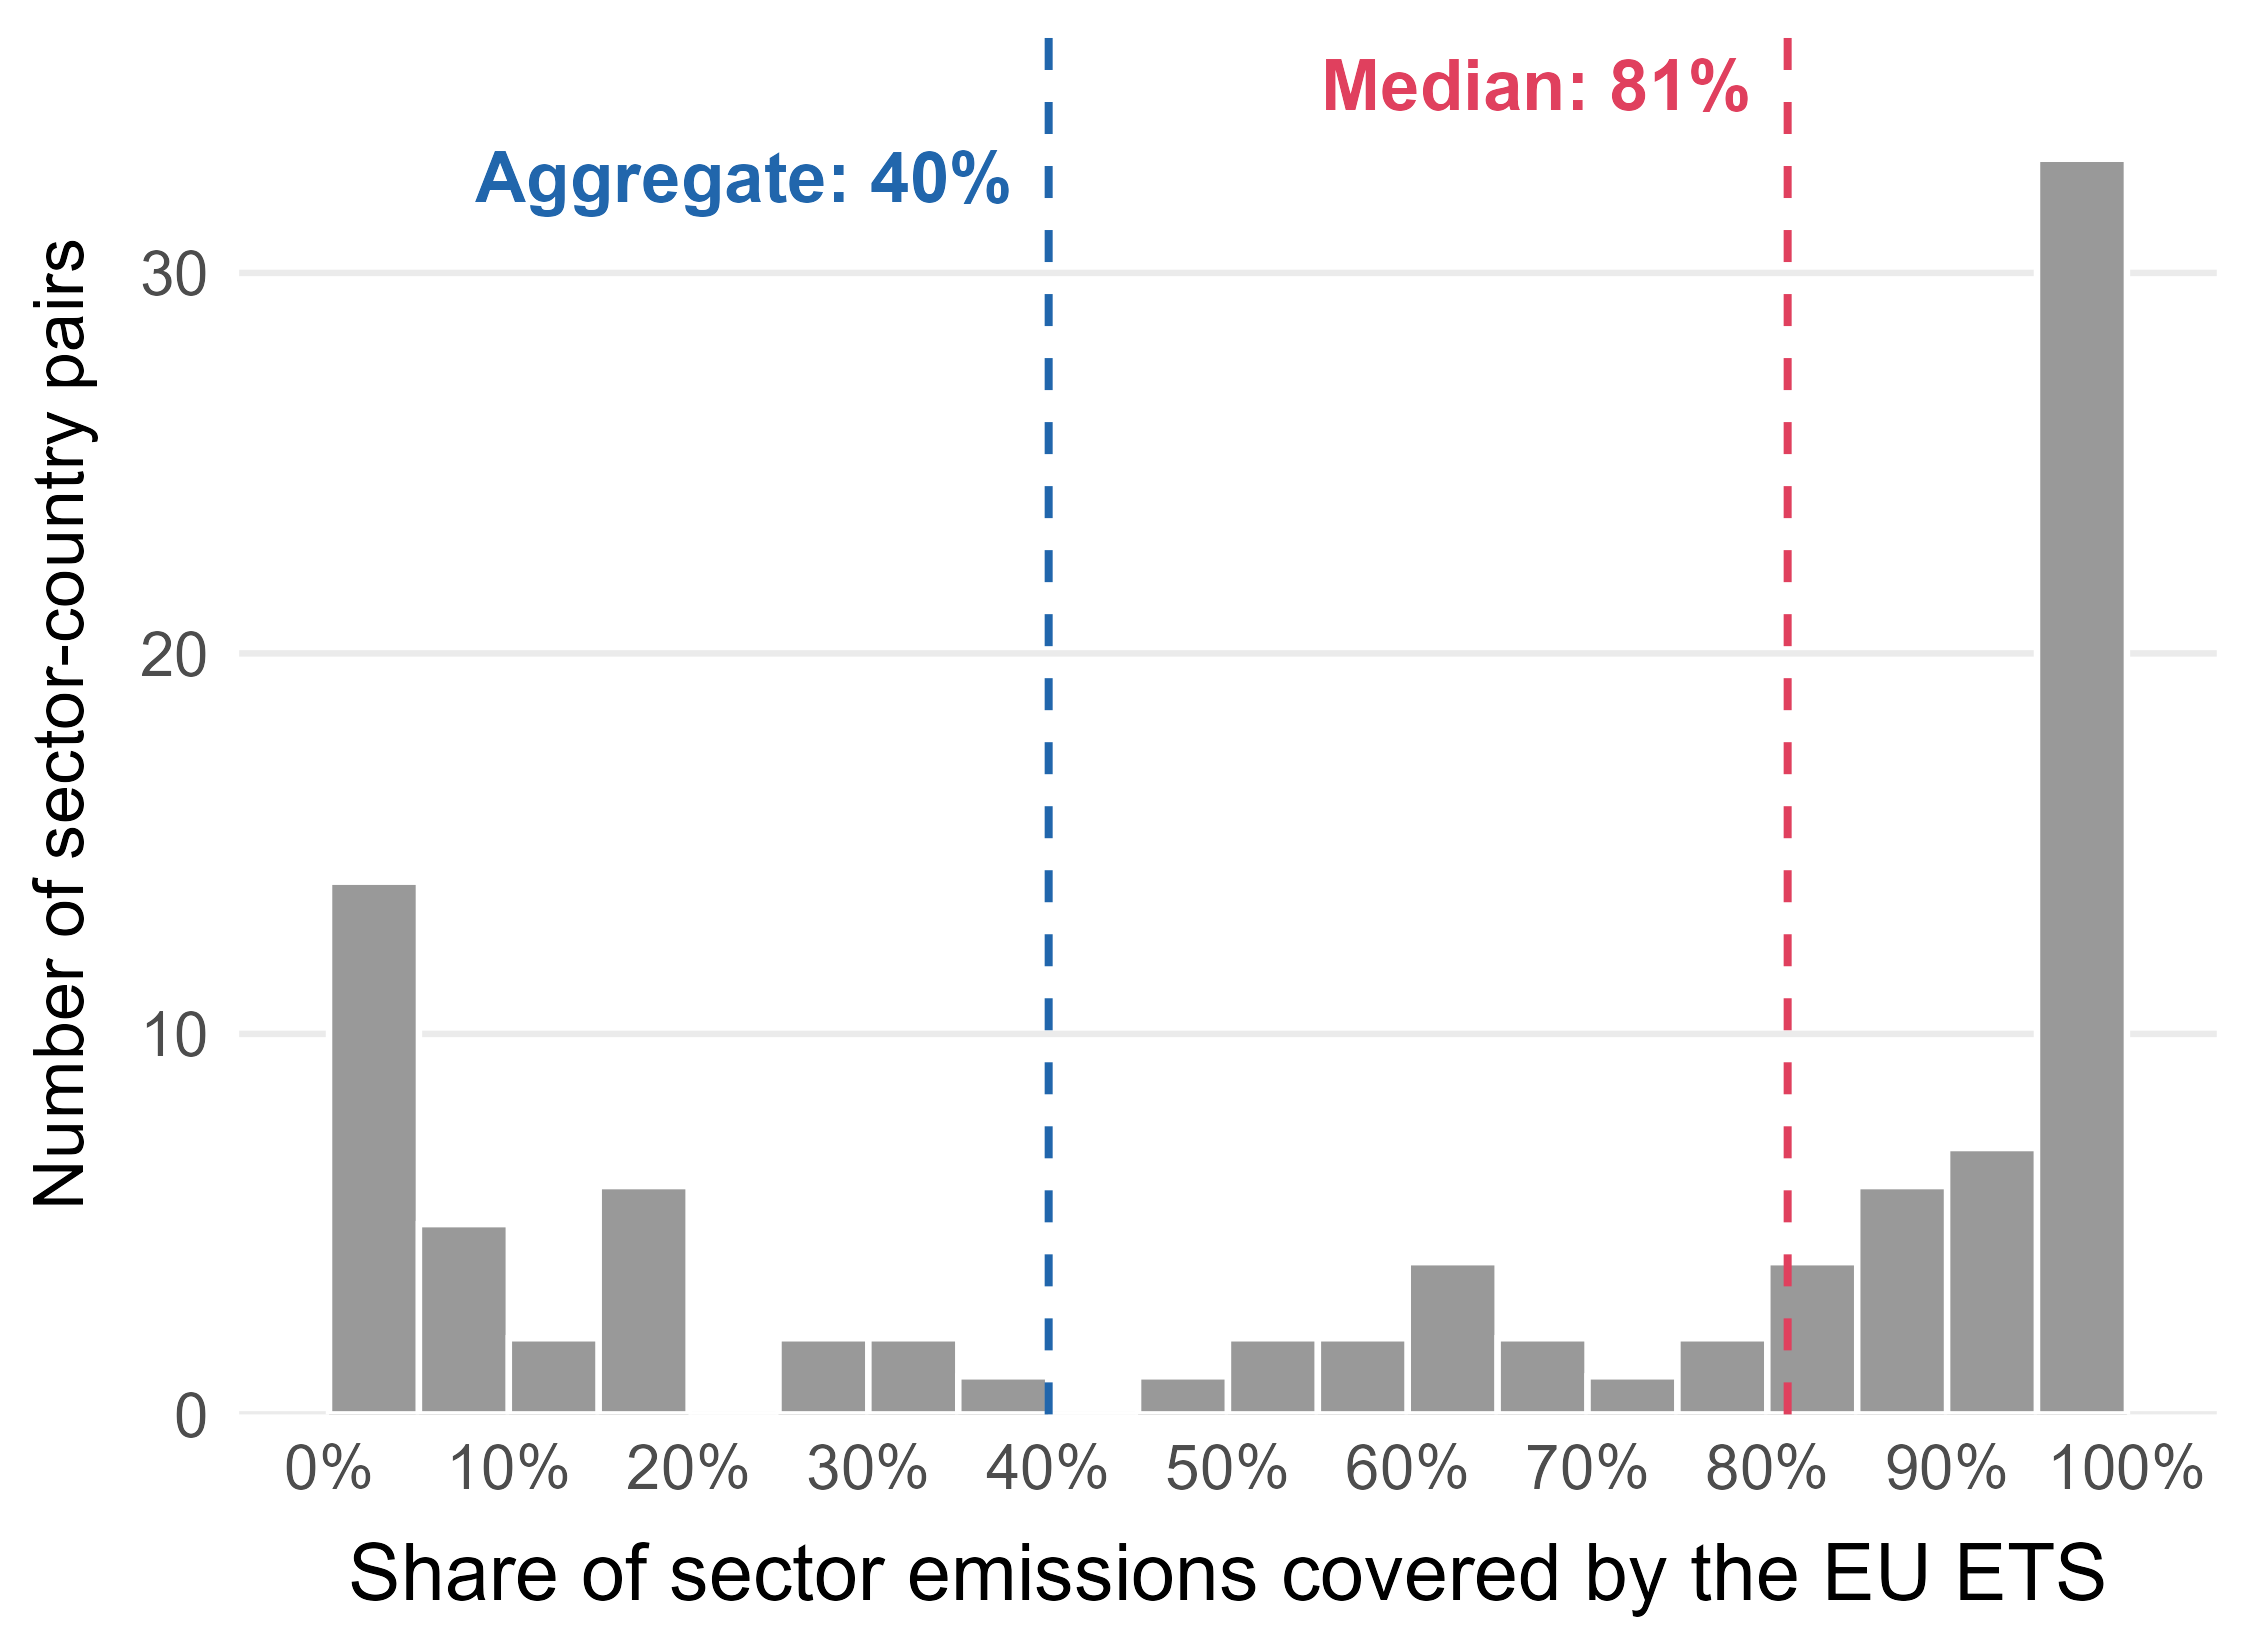
\includegraphics[width=0.99\linewidth]{figures/panel_c_within_sector_coverage.png}
        \end{figure}
    \end{column}
    \begin{column}{0.42\textwidth}
        \begin{wideitemize}
            \item $\sim$75 carbon-pricing instruments in 2024, $\sim$\alertb{a quarter} of global emissions
            \item Coverage is \alerto{partial and uneven} across \emph{and} within sectors
            \item EU ETS: median targeted sector $\sim$80\% priced, but only $\sim$\alertr{40\%} of emissions priced in aggregate
            \item[] \alertg{$\Rightarrow$} incompleteness is the rule, not the exception
        \end{wideitemize}
    \end{column}
    \end{columns}

\end{frame}

%%%%%%%%%%%%%%%%%%%%% MOTIVATION 2: WHY NETWORK %%%%%%%%%%%%%%%%%%%%%%%%%
\begin{frame}{Why the production network matters}

    Three questions: \alertb{(1)} effect of a scheme on aggregate emissions?
    \alertb{(2)} how does it depend on \emph{who} is covered?
    \alertb{(3)} is there a firm whose coverage reduces emissions most?

    \vspace{0.3cm}
    \begin{wideitemize}
        \item A firm's emissions are partly \alertp{its own}, partly \alerto{embodied in the inputs it buys}
        \begin{wideitemize}
            \item[\alertp{1.}] \alertp{Who is exposed} to a carbon price is a network object (taxing one firm reaches beyond it)
            \item[\alerto{2.}] The \alerto{aggregate effect} depends on where dirty firms sit in the network
        \end{wideitemize}
        \item[] The object that matters: \alertg{network-adjusted emission intensity}
        $$ \Psi_e := \Psi\,\overline{\mathcal{E}}, \qquad \Psi = (I-\Omega)^{-1} \quad \text{(direct $+$ upstream-embodied; scope 1$+$2$+$3)} $$
    \end{wideitemize}

\end{frame}

%%%%%%%%%%%%%%%%%%%%% ENVIRONMENT / SETUP %%%%%%%%%%%%%%%%%%%%%%%%%%%%%%%
\begin{frame}{Environment}

    \begin{wideitemize}
        \item Closed economy: household, government, $N$ producers (CRS, marginal-cost pricing $p_i=mc_i$)

        \item \alertb{Policy}: carbon price $p_z$ and coverage vector $\tau=\{\tau_i\}$, $\tau_i\in\{0,1\}$

        \item Producer $i$: Cobb--Douglas in labor and a \alertp{nested-CES} input bundle
        \begin{wideitemize}
            \item[-] across sectors $\sigma_B$ (weak substitution), within sector $\sigma_W$ (stronger)
        \end{wideitemize}

        \item \alertg{Network objects}: input--output matrix $\Omega$, Domar weights $\lambda_i$, Leontief inverse $\Psi=(I-\Omega)^{-1}$

        \item Emissions a by-product of production: $z_i = e_i f_i$, intensity $\overline{e}_i$ in the no-policy economy
    \end{wideitemize}

\end{frame}

%%%%%%%%%%%%%%%%%%%%% ABATEMENT / TECHNIQUE %%%%%%%%%%%%%%%%%%%%%%%%%%%%%
\begin{frame}{Firms abate: the technique channel}

    \begin{wideitemize}
        \item A covered firm pays $p_z$ per unit of emissions $\Rightarrow$ it \alertb{abates}: chooses effort $\kappa_i$
        $$ e_i = (1-\kappa_i)^{\alpha_i}\,\overline{e}_i $$
        {\small $\alpha_i$ governs \alerto{how hard firm $i$ is to abate} (disciplined from abatement-elasticity estimates)}

        \item To first order, the \alertp{technique response}:
        $$ \frac{d \log e_i}{d p_z}\bigg|_{p_z=0} = -\,\tau_i\,\alpha_i^2\,\overline{e}_i \;<\;0 $$

        \item \alertg{Key separability}: abatement lowers intensity but leaves the firm's \emph{input mix} (hence pass-through) unchanged to first order
    \end{wideitemize}

\end{frame}

%%%%%%%%%%%%%%%%%%%%% PRICE PROPAGATION %%%%%%%%%%%%%%%%%%%%%%%%%%%%%%%%%
\begin{frame}{The carbon price propagates through prices}

    \begin{wideitemize}
        \item Each firm passes its carbon cost into its price; buyers inherit it through their inputs:
        $$ \frac{d \log p_i}{d p_z} = \sum_{j\in\N}\Omega_{ij}\,\frac{d \log p_j}{d p_z} \;+\; \Omega_{iL}\,\frac{d \log w}{d p_z} \;+\; \tau_i\,\overline{e}_i $$

        \item In matrix form (the \alertb{exposure} of every price to the policy):
        $$ \frac{d \log \mathbf{p}}{d p_z} = \Psi\,(\tau \circ \overline{\mathcal{E}}) \;+\; \Psi_{(:,L)}\frac{d \log \lambda_L}{d p_z} $$

        \item[] \alertg{$\Rightarrow$} a firm's exposure is its \emph{covered, network-weighted} upstream emission content --- itself a $\Psi$ object
    \end{wideitemize}

\end{frame}

%%%%%%%%%%%%%%%%%%%%% THREE-CHANNEL DECOMPOSITION %%%%%%%%%%%%%%%%%%%%%%%
\begin{frame}{Decomposition: scale, technique, reallocation}

    \begin{wideitemize}
        \item Aggregate emissions move through three channels (Grossman--Krueger accounting, mapped to primitives):
        $$ \frac{d \log Z}{d p_z}\bigg|_{0}
            = \underbrace{\sum_{i\in\N}\frac{z_i}{Z}\frac{d\log e_i}{d p_z}}_{\text{\alertp{technique (abatement)}}}
            \;+\; \underbrace{\sum_{i\in\N}\frac{z_i}{Z}\Big[\tfrac{d\log\lambda_i}{d p_z}-\tfrac{d\log p_i}{d p_z}\Big]}_{\text{\alertb{reallocation}}} $$

        \item \alerto{Scale} $\approx 0$: by Hulten, $\dfrac{d\log Y}{d p_z}\Big|_{0}=0$ --- to first order the policy is a pure pollution-cutting device, not an output story

        \item \alertp{Technique} is set by \emph{covered} firms; \alertb{reallocation} is where the network enters
    \end{wideitemize}

\end{frame}

%%%%%%%%%%%%%%%%%%%%% THE THEOREM %%%%%%%%%%%%%%%%%%%%%%%%%%%%%%%%%%%%%%%%
\begin{frame}{Main result: a sufficient-statistic decomposition}

    \begin{tcolorbox}[colback=blue!4,colframe=blue!45!black]
    $$ \frac{d \log Z}{d p_z}\bigg|_{p_z=0}
        = \underbrace{-\sum_{i \in \N} \frac{\tau_i z_i}{Z}\,\alpha_i^2\,\overline{e}_i}_{\text{\alertp{technique} $<0$, covered firms}}
        \;\underbrace{-\,\sigma \sum_{i \in \N \cup \{C\}} \frac{x_i}{Z}\,\mathbb{C}_{\Omega_{(i,:)}}\!\left(\frac{d \log \mathbf{p}}{d p_z},\,\Psi_e\right)}_{\text{\alertb{reallocation}: one covariance}} $$
    \end{tcolorbox}

    \begin{wideitemize}
        \item Across each buyer's inputs: covariance between \alertb{exposure} ($\tfrac{d\log\mathbf p}{dp_z}$) and \alertg{network-adjusted intensity} $\Psi_e$
        \item Its \alertr{sign} decides whether the network \alertg{amplifies} ($\mathbb{C}>0$) or \alerto{leaks} ($\mathbb{C}<0$)
        \item $(1-\sigma)$ governs the \alertp{magnitude}, not the sign
        \item[] \alertr{Complete coverage} ($\tau=\mathbf 1$): covariance $\to$ \alertg{variance} $\Rightarrow$ reallocation \emph{always} amplifies
    \end{wideitemize}

\end{frame}

%%%%%%%%%%%%%%%%%%%%% EMISSION CENTRALITY %%%%%%%%%%%%%%%%%%%%%%%%%%%%%%%
\begin{frame}{Whom to cover? Emission centrality}

    \begin{wideitemize}
        \item The decomposition is \alertb{additively separable} across covered firms $\Rightarrow$ define the marginal value of covering firm $j$ alone:
        $$ \text{Centrality}_j \;=\; -\frac{z_j}{Z}\,\alpha_j^2\,\overline{e}_j
            \;-\; \sigma \sum_{i \in \N \cup \{C\}} \frac{x_i}{Z}\,\mathbb{C}_{\Omega_{(i,:)}}\!\Big(\Psi_{(:,j)}\,\overline{e}_j,\ \Psi_e\Big) $$

        \item \alertp{Own-abatement} term ($z_j$, $\overline e_j$) $+$ a \alertb{network-position} term
        \item This is the object counterfactuals \alertg{rank firms on} --- and it makes the network's value an \emph{empirical} question
    \end{wideitemize}

\end{frame}

%%%%%%%%%%%%%%%%%%%%% FACTS THAT DISCIPLINE %%%%%%%%%%%%%%%%%%%%%%%%%%%%%%
\begin{frame}{Taking it to Belgian data: facts that discipline the model}

    \begin{columns}
    \begin{column}{0.5\textwidth}
        \begin{figure}
            \centering
            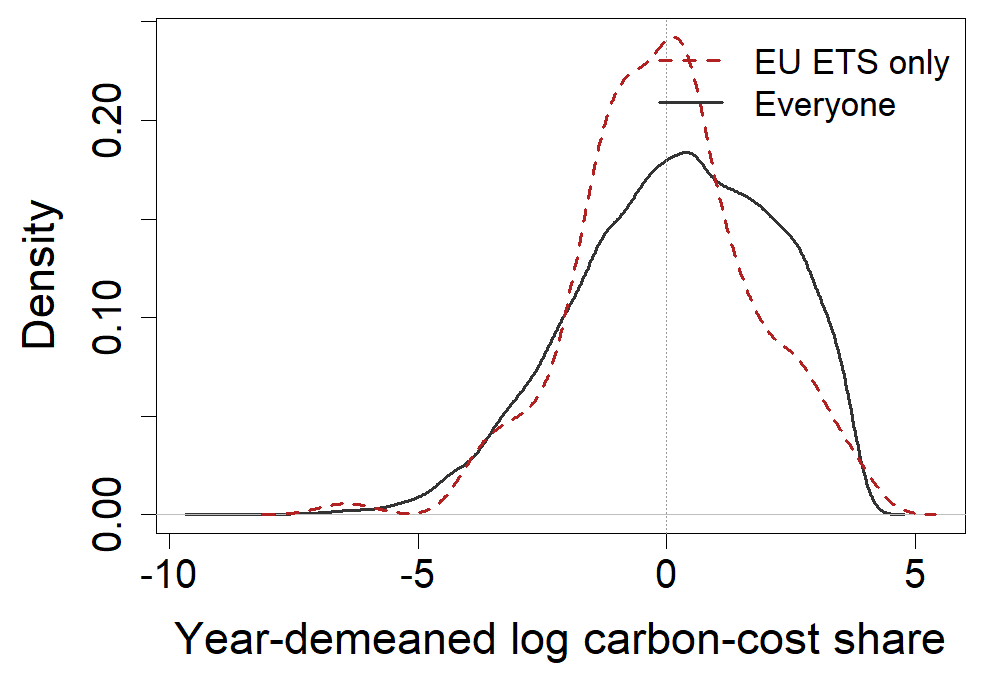
\includegraphics[width=0.92\linewidth]{figures/emission_cost_share_firm_p80.png}
        \end{figure}
    \end{column}
    \begin{column}{0.5\textwidth}
        \begin{wideitemize}
            \item At $p_z=80$: median emitter's carbon cost $\approx$ \alertb{2.5\%} of total cost; $\sim$1 in 6 exceed 20\%
            \item Wide \alerto{dispersion} in direct intensity: within (4d, year) $p_{90}/p_{10}\!\approx\!5.7$; $\to\!\sim$30-fold with the imputed tail
            \item Direct $\leftrightarrow$ upstream link is \alertr{weak} (Spearman $0.24$--$0.33$)
            \item For \alertb{1 in 3} ETS firm-years, \emph{upstream} emissions exceed own direct
        \end{wideitemize}
    \end{column}
    \end{columns}

    \vspace{0.1cm}
    {\footnotesize Thin within-sector supplier base ($\sim$1.5 suppliers/sector) vs.\ broad across-sector base ($\sim$25 sectors sourced) $\Rightarrow$ $\sigma_W>\sigma_B$.}

\end{frame}

%%%%%%%%%%%%%%%%%%%%% CALIBRATION %%%%%%%%%%%%%%%%%%%%%%%%%%%%%%%%%%%%%%%%
\begin{frame}{Calibration}

    \begin{wideitemize}
        \item 2019 Belgian firm-level network ($\Omega$, $\lambda$) from B2B $+$ imports $+$ balance sheets; intensities $\overline{\mathcal E}$ from EUTL ($+$ imputation for the non-ETS tail)

        \item Realized \alertb{EU ETS} coverage $\tau$; carbon price $p_z = $ \alerto{80 EUR/t} (2022 EUA)

        \item Benchmark elasticities:
        $$ \sigma_B = 0.1, \qquad \sigma_W = 2.5, \qquad \rho = 0.7, \qquad \alpha = 2 $$
        {\small ($\rho$: incomplete pass-through, a Katz--Bonacich Leontief $\Psi_\rho$; $\alpha$ from abatement-elasticity estimates. Robustness over grids on each.)}
    \end{wideitemize}

\end{frame}

%%%%%%%%%%%%%%%%%%%%% RESULT 1: EU ETS DECOMP %%%%%%%%%%%%%%%%%%%%%%%%%%%
\begin{frame}{Result 1 --- the EU ETS effect is mostly abatement}

    \begin{center}
    \begin{tabular}{lcc}
    \toprule
    Channel & $\Delta\log Z$ & share \\
    \midrule
    \textbf{Total}            & \alertb{$-0.421$} & \\
    \quad Scale               & $-0.000$ & $\approx 0$ \\
    \quad \alertp{Technique}  & \alertp{$-0.371$} & $\approx 88\%$ (\,$\sim$7/8\,) \\
    \quad \alertb{Composition}& \alertb{$-0.049$} & $\approx 12\%$ \\
    \bottomrule
    \end{tabular}
    \end{center}

    \begin{wideitemize}
        \item Composition is \alertg{negative} $\Rightarrow$ the Belgian network \alertg{amplifies} abatement (covariance positive: covered firms are positioned in cleaner-leaning supply chains)
        \item But \alerto{uneven}: taxing a firm lowers emissions at \alertb{$\sim$4 in 5} firms, raises them at the rest --- the raisers offset \alertr{$\sim$1/5} of the reductions
        \item For \alertr{$\sim$1 in 25} firms, coverage \emph{backfires}: demand shifts to dirtier uncovered rivals
    \end{wideitemize}

\end{frame}

%%%%%%%%%%%%%%%%%%%%% RESULT 2: WHICH VS HOW MANY %%%%%%%%%%%%%%%%%%%%%%%
\begin{frame}{Result 2 --- \emph{which} firms beats \emph{how many}}

    \begin{columns}
    \begin{column}{0.44\textwidth}
        \begin{figure}
            \centering
            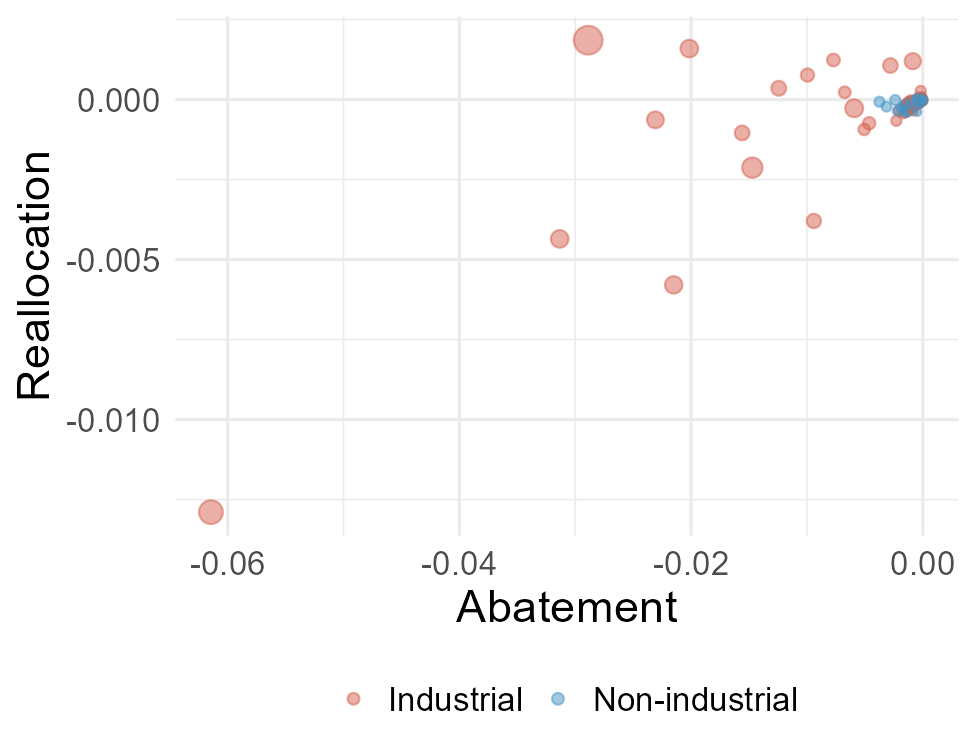
\includegraphics[width=0.86\linewidth]{figures/centrality_plane.png}
        \end{figure}
        {\scriptsize Technique vs.\ composition centrality (corr.\ $0.74$).}
    \end{column}
    \begin{column}{0.56\textwidth}
        \begin{wideitemize}
            \item Re-selecting the \emph{same number} of firms toward central ones: \alertg{$+31.7\%$} vs.\ ETS
            \item Expanding to \emph{all} of industry: only \alerto{$+5.3\%$}
            \item[] \alertb{$\Rightarrow$ \emph{which} $\approx$ 6$\times$ \emph{how many}}
        \end{wideitemize}
    \end{column}
    \end{columns}

    \begin{tcolorbox}[colback=blue!4,colframe=blue!45!black,boxsep=2pt,top=3pt,bottom=3pt]
    \footnotesize \textbf{But:} holding firm count fixed, ranking on \alertr{direct emissions $z_i$ alone}
    recovers \alertr{$\sim$94\%} of the centrality gain --- the network's extra value sits at the
    \emph{backfiring} margin, not in everyday selection.
    \end{tcolorbox}

\end{frame}

%%%%%%%%%%%%%%%%%%%%% CONCLUSION %%%%%%%%%%%%%%%%%%%%%%%%%%%%%%%%%%%%%%%%%
\begin{frame}{Chapter 3 --- takeaways}

    \begin{wideitemize}
        \item A \alertb{transparent decomposition} of targeted carbon pricing in a network: scale ($\approx 0$), technique, and reallocation --- the last a \alertg{single covariance} of exposure with network-adjusted intensity $\Psi_e$

        \item Empirically (Belgium, EU ETS): the cut is \alertp{$\sim$7/8 abatement}; the network \alertg{amplifies} modestly

        \item The network is indispensable for \alertb{diagnosis} --- measuring the effect and flagging the $\sim$1-in-25 firms that backfire --- but for \alerto{selection} a constrained regulator simply \alertr{targets the heaviest emitters}

        \item[] \alertp{Next}: open economy (cross-border leakage --- Chapter~2), and the jointly-optimal covered set
    \end{wideitemize}

\end{frame}


%%%%%%%%%%%%%%%%%%%%%%%%%%%%%%%%%%%%%%%%%%%%%%%%%%%%%%%%%%%%%%%%%%%%%%%%%%
%%  THANK YOU
%%%%%%%%%%%%%%%%%%%%%%%%%%%%%%%%%%%%%%%%%%%%%%%%%%%%%%%%%%%%%%%%%%%%%%%%%%
\begin{frame}[plain]
    \begin{center}
        \vspace{1.5cm}
        {\Huge \textbf{Thank you!}}\\[1cm]
        {\large gabrielj@u.northwestern.edu}
    \end{center}
\end{frame}

\end{document}
